\chapter{Methods}\label{chapter:methods}
\section{Experiment}\label{sec:experiment}
To accurately determine the characterstic parameters of a VECSEL chip, a setup is required that can measure a small change of the reflectivity over a dynamic range of about 4 order of magnitde in pulse fluence. Such a setup has ben build and used by and is shown in.


\section{VECSEL Chips}

\subsection{Experimental setup}\label{subsection:set-up}
The pulsed laser is a modelocked Ti:sapphire laser, emitting femtosecond pulses at \SI{810}{\nm} with a repetion rate of \SI{80}{\MHz} and an average output power of \SI{4}{\W}. The beam then passes through an optical parametric oscillator, where a nonlinear crystal is used to split the beam in an idler and signal wave. Reduced the max output power to \SI{650}{\mW}. The idler has been tuned to \SI{2071.7}{\nm} and was kept there by an automeded feedback loop 

To achieve a wide dynamic range of pulse fluences, the beam passes through two wire-grid polarizers where one is placed on a controllable rotation stage. To control attenuation.   

\subsubsection{Automation of the pump power}{\label{subsubsection:pump}}
\subsubsection{Signal trace analysis}{\label{subsubsection:signal}}
\begin{figure}[h]
    \centering
    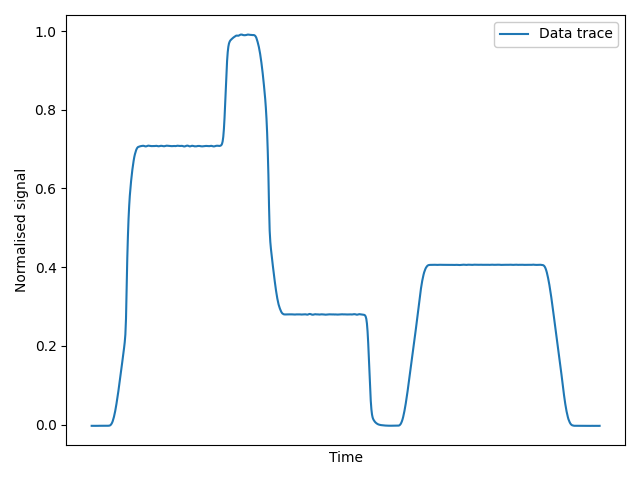
\includegraphics[width=8cm]{images/trace1.png}
\end{figure}
\section{Data processing}\label{sec:processing}


